\section{Results from Experiments}\label{sec:expresults}
After all experiments were conducted using the implementations described in Section \ref{sec:implmltech} the results were converted into \textbf{pandas’} dataframes and later outputted as shown in Table \ref{table:imp_os_ex}, with the metrics described in Section \ref{sec:perf_metrics}. Table \ref{table:imp_os_ex} just shows a snippet of the dataframe where in total 30 rows (each model with two different imputation techniques for the five forecasting periods) were shown. This process was then done for each experiment described in Section \ref{sec:carriedexp}, so in the end four \textbf{panda’s} dataframes were outputted. 
\begin{table}[H]
\centering
  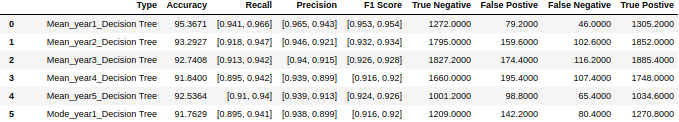
\includegraphics[scale = .7]{imgs/imp_os_pp.png}
  \caption{A snippet for results for Experiment 1 (From First Principles)}
  \label{table:imp_os_ex}
\end{table}
\noindent Based on the results which were described above, the confusion matrix and ROC curve were plotted as shown in Figure \ref{fig:pp_plots_results}, for the best performing forecasting period (\nth{1} year), model (Decision Tree) and imputation technique (Mean). 
\begin{figure}[H]
\centering
  \begin{subfigure}[b]{0.5\textwidth}
    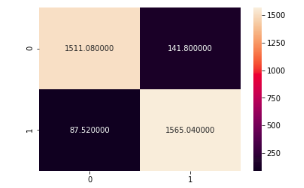
\includegraphics[scale = .7]{imgs/confusion_matrix_1.png}
    \caption{Confusion Matrix}
  \label{fig:confusion_matrix_pp}
  \end{subfigure}
  %
  \begin{subfigure}[b]{0.4\textwidth}
    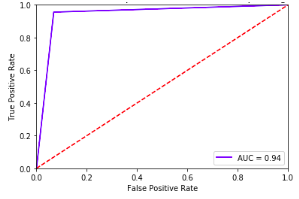
\includegraphics[scale = .9]{imgs/mean_imp_y1_pp_roc.png}
  \caption{ROC curve}
  \label{fig:roc_pp}
  \end{subfigure}
  \caption{Plots for best performing Model (Decision Tree) using best imputation technique (Mean); Confusion Matrix using averaged values of all forecasting periods and ROC curve for best forecasting period (\nth{1} Year) using first principles}
  \label{fig:pp_plots_results}
\end{figure}
\noindent Following the first step to output the results (each model using different imputation techniques for every forecasting period for four experiments), all the results were averaged by the forecasting periods to get a better metric for comparison. Table \ref{table:mean_metrics_pp} shows the averaged results for each model and experiment.   
\begin{table}[H]
\centering
  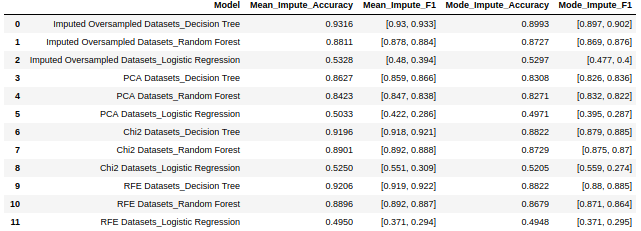
\includegraphics[scale = .7]{imgs/mean_metrics_pp.png}
  \caption{The mean results (forecasting periods) for each Experiment (From First Principles)}
  \label{table:mean_metrics_pp}
\end{table}